\chapter{Discussions}

\section{Future Work} 
 In this study, we utilized a Transformer-based framework called Paint 
Transformer \cite{liu2021paint} for transforming the content of the input image 
to match the brush style of a reference image.
Our model used the Paint Transformer as is, to train a stroke prediction model, 
and therefore, the brush parameters were the same as the original, including 5 
shape parameters and 3 color parameters. However, we believe that adding more 
parameters could make the stroke expression more flexible in future works.
Accordingly, it is also necessary to rethink the loss function for brush style 
comparisons.

In the model we introduced in this paper, each stroke in the painting is created 
by simply adjusting the size of the brush image, as shown in Figure \ref{strokeparams}.
However, there is another technique that can be used to create brushstrokes 
- repeating the same brush image multiple times in succession.
For example, in a painting software Clip Studio \cite{clipstudio}, it is 
possible to draw strokes like in Figure \ref{goodstroke}.
\begin{figure}[h]
    \centering
    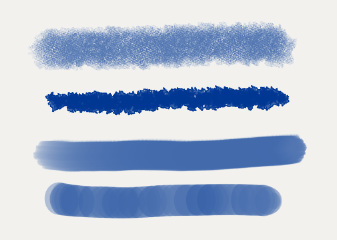
\includegraphics[width=63truemm]{resources/6_discussions/strokes-clipstudio.png}
    \caption{
        Strokes drawn in Clip Studio.
    }
    \label{goodstroke}
\end{figure}
\newline
These types of strokes cannot be created simply by extending the base brush 
image. Although these strokes are created by various settings such as repeating 
pattern, spacing between the repetition, and strength of brush entry and exit, 
it would be possible to increase the expression of the strokes with just 
expressing the strokes as the simple repetition of the base brush image.
For example, using brush (e) and (f) in Figure \ref{Brushes} as the base brush, the 
generated brush stroke shown in Figure \ref{results} is unnatural, and this is 
believed to be because the strokes are represented by scaling the base image. 
If the expressiveness of the brush is increased, believed that the model generate 
strokes like in the Figure \ref{stroke-shouldbe}. As a result, it is expected 
that more natural images can be generated. 
Additionally, in the original stroke expression, the color is monochrome, 
but it is expected that the expressiveness will increase by making it possible 
to express the gradation.

\begin{figure}[h]
    \centering
    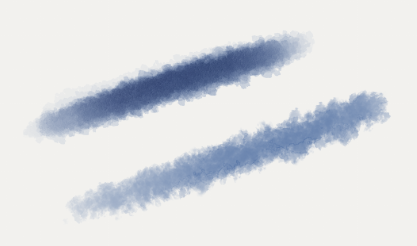
\includegraphics[width=100truemm]{resources/6_discussions/coral_cloud.png}
    \caption{
        Strokes that would be depicted by brushes (e) and (f) in Figure \ref{Brushes},
        drawn in Clip Studio.
    }
    \label{stroke-shouldbe}
\end{figure}


By increasing the brush parameters, it is expected that the stroke expression 
can be made more flexible and the result picture generated by the model will 
be better.
Furthermore, various extensions such as the ability to draw curved strokes and 
consideration for blending color of strokes can also be considered in addition 
to the above discussion.

\section{Conclusion}
 In this research, we introduced a novel approach that utilizes FNNs to 
transform the content of the input image to match the brush style of a 
reference image.
To achieve this, we prepared multiple brush images used to generate the strokes.
Our ultimate goal is to produce strokes that closely emulate the brush style of 
the reference image, however, our current research is still far from achieving 
this goal due to the inflexibility of the strokes, including the small number 
of stroke parameters. There is still room for improvement in the way strokes 
are expressed, and it is expected that the accuracy of mimicking brush style 
will improve with these improvements.